\documentclass{article}
\usepackage{graphicx} % Required for inserting images
\usepackage[UTF8]{ctex}

\title{afterclass-practice 0830}
\author{danica Lu}
\date{August 2026}

\begin{document}

\maketitle

\section{练习1}
\begin{tabular}{l|r|r}
Item & Quantity & Price(\$)\\
\hline
Nails & 500 & 0.34\\
Wooden borads & 100 & 4.00\\
Bricks & 240 & 11.50\\
\end{tabular}

\begin{tabular}{l|ccc}
& Year & &\\
\cline{2-4}
City & 2006 & 2007 & 2008\\
\hline
London & 45789 & 46551 & 51298\\
Berlin & 34539 & 32543 & 29870\\
Paris & 49835 & 51009 & 51970\\
\end{tabular}

\section{练习2-练习7}
\begin{eqnarray}
     e & = & mc^2\\ 
     \pi & = & \frac{c}d{}\\
     \frac{d}{dx}e^x & = & e^x \\
     \frac{d}{dx}\int_0^\infty f(s)ds
      & = & f(x)\\
      f(x) &= & \sum_i 0^\infty \frac{f^{(i)}(0)}{i!}x^i\\
      x& = & \sqrt{\frac{x_i}{z}y}
\end{eqnarray}

\section{练习8}
\begin{figure}[h!]
  \centering
  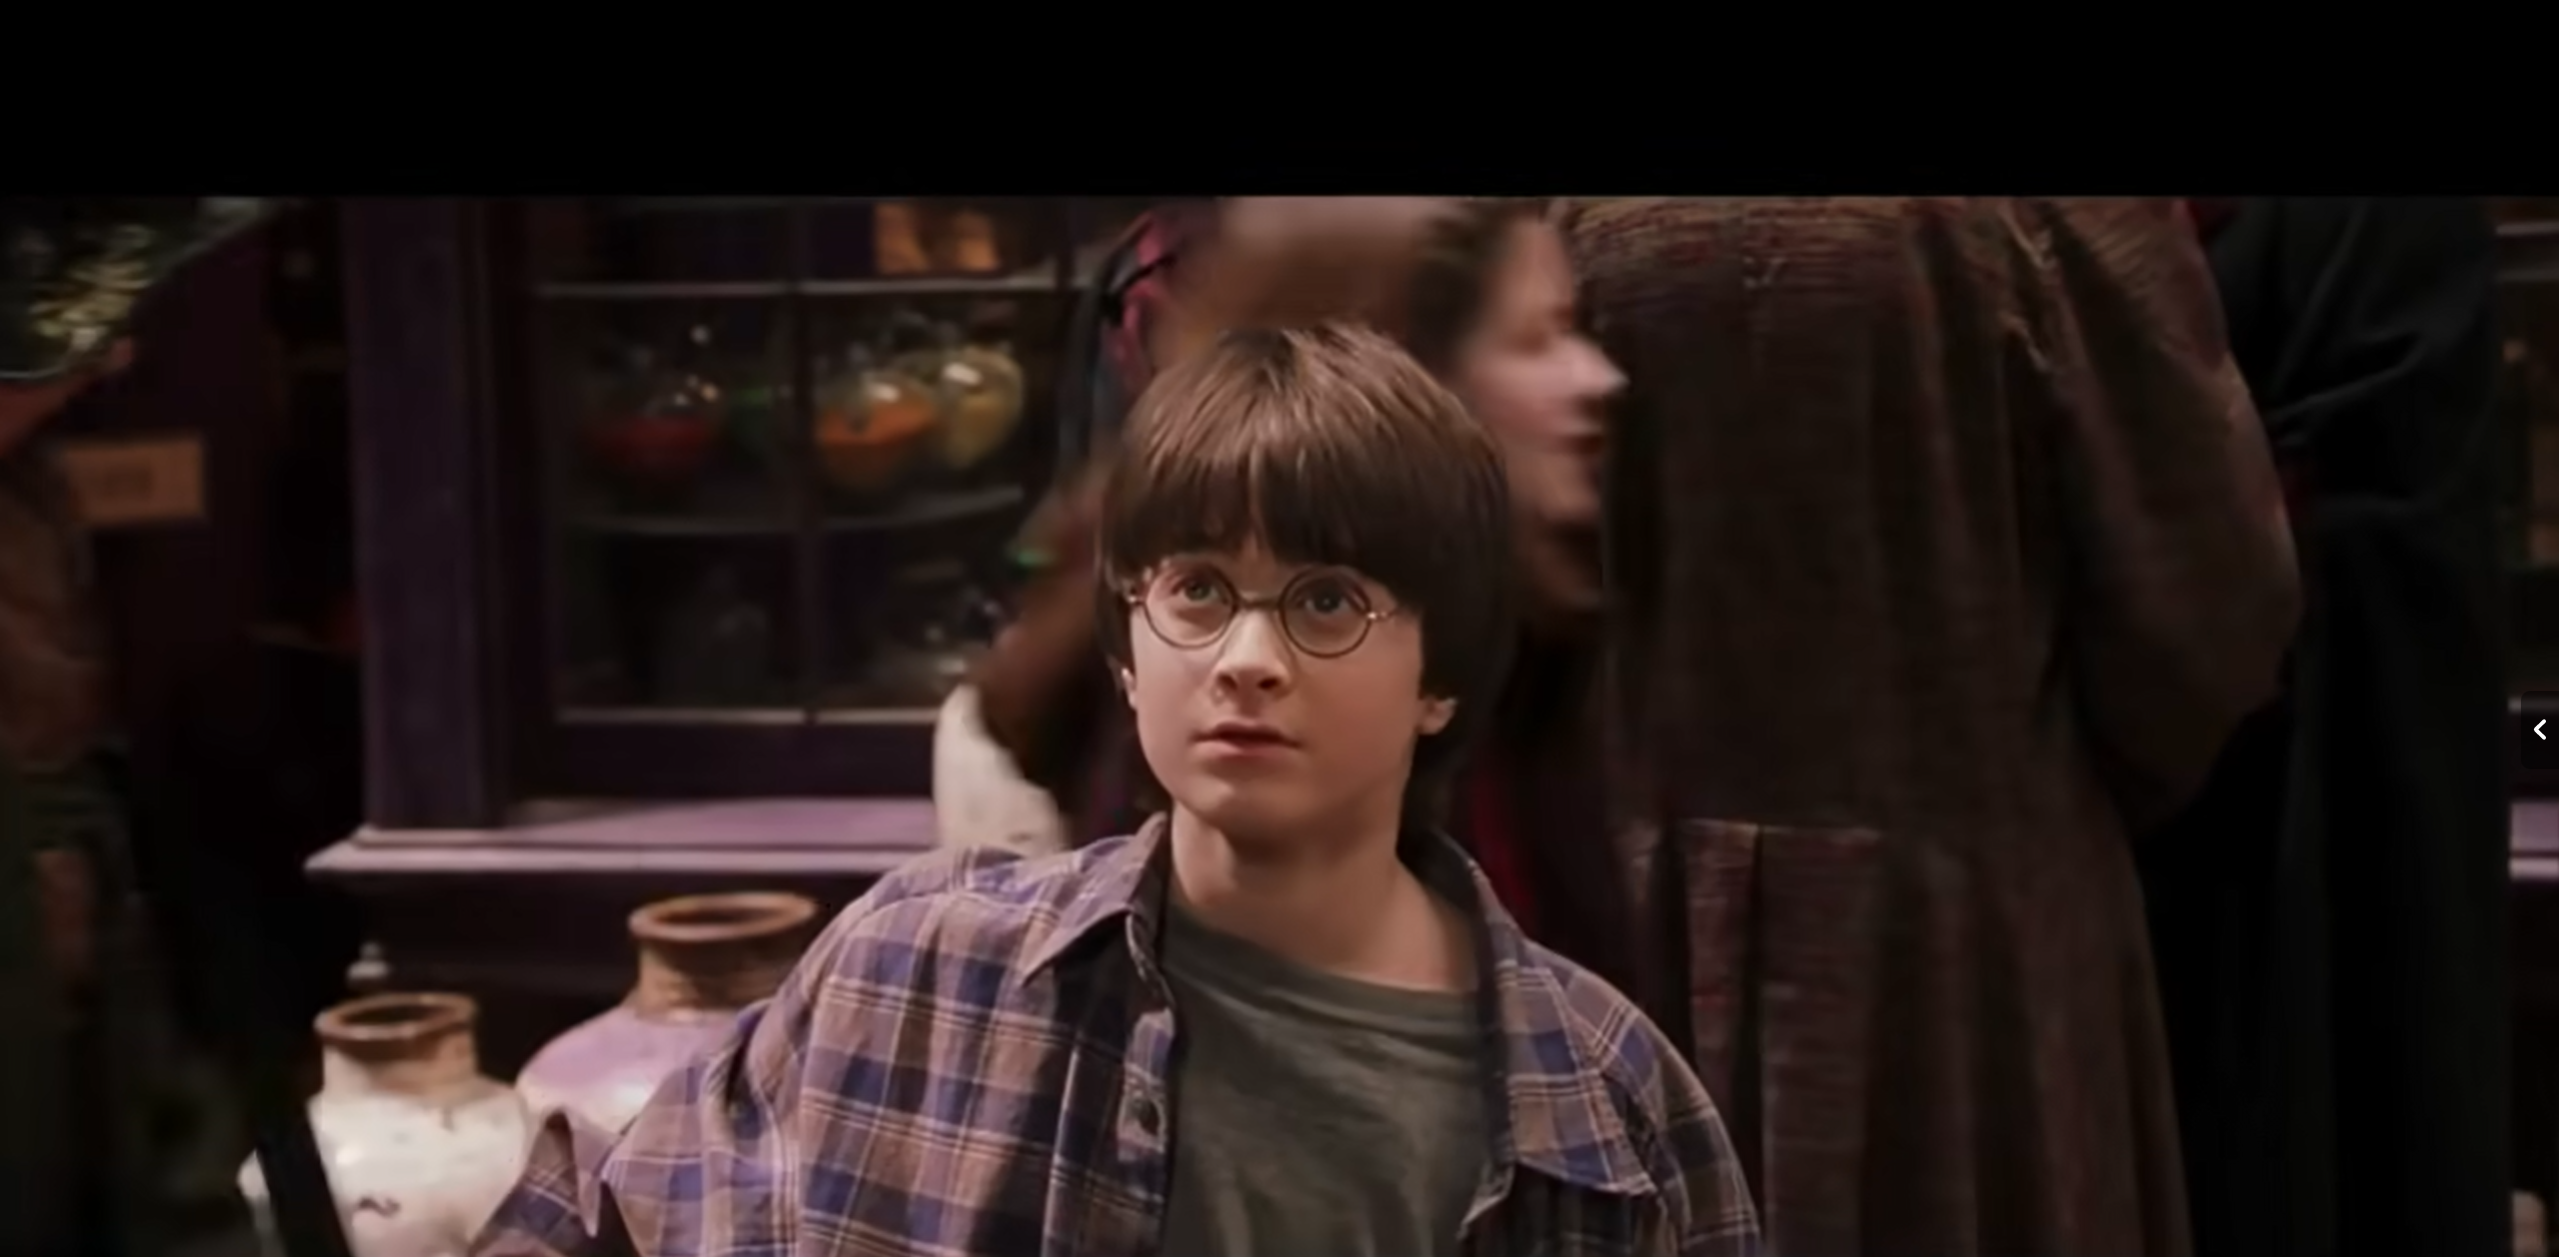
\includegraphics[width=1\textwidth]{屏幕截图 2025-10-17 161352.png}
  \caption{My test image}
\end{figure}
   
\section{练习9}
\documentclass{article}
\begin{document}

J.K.Rowling写了哈利波特\cite{Rowling2007}。
DanicaLu即将写一篇ccf-a论文\cite{danica2027}。

\bibliographystyle{plain}
\bibliography{references}

\section{练习10}
\begin{itemize}
    \item[+]sth positive
    \item[-]sth negative
    \item sth
     \begin{itemize}
         \item sub-sth
         \item other
     \end{itemize}
\end{itemize}

\end{document}


\end{document}
